% !TEX root =  ../pers_schedules.tex

\section{Demonstration of Personalized Schedules}
\label{sec : pers_schedule_PRIAS}
To demonstrate how the personalized schedules work, we apply them to the patients enrolled in PRIAS study. To this end, we divide the PRIAS dataset into a training dataset with 5264 patients and a demonstration dataset with three patients who never experienced GR. We fit a joint model to the training dataset and then use it to create personalized schedules for patients in demonstration dataset. We fit the joint model using the R package \textbf{JMbayes} \citep{rizopoulosJMbayes}, which uses the Bayesian methodology to estimate the model parameters.

\subsection{Fitting the Joint Model to PRIAS Dataset}
\label{subsec : jm_fit_prias}
The training dataset contains age at the time of inclusion in PRIAS, PSA levels and the time interval in which GR is detected, for 5264 prostate cancer patients. PSA was measured at every three months for the first two years and every six months thereafter. To detect GR, biopsies were conducted as per the PRIAS schedule (Section \ref{sec : introduction}). For the longitudinal analysis of PSA we use $\log_2 \mbox{PSA}$ measurements instead of the raw data \citep{nieboer2015nonlinear}. The longitudinal sub-model of the joint model we fit is given by:
\begin{equation}
\label{eq : long_model_prias}
\begin{aligned}
\log_2 \mbox{PSA}(t) &= \beta_0 + \beta_1 (\mbox{Age}-70) + \beta_2 (\mbox{Age}-70)^2 + \sum_{k=1}^4 \beta_{k+2} B_k(t,\mathcal{K})\\ 
&+  b_{i0} + b_{i1} B_7(t, 0.1) + b_{i2} B_8(t, 0.1) +
\varepsilon_i(t).
\end{aligned}
\end{equation}
where $B_k(t, \mathcal{K})$ denotes the $k$-th basis function of a B-spline with three internal knots at $\mathcal{K} =\{0.1, 0.5, 4\}$ years, and boundary knots at zero and seven (0.99 quantile of the observed follow-up times) years. The spline for the random effects consists of one internal knot at 0.1 years and boundary knots at zero and seven years. The choice of knots was based on exploratory analysis as well as on model selection criteria AIC and BIC. Age of patients was median centered to avoid numerical instabilities during parameter estimation. For the relative risk sub-model the hazard function we fit is given by:
\begin{equation}
\label{eq : hazard_prias}
h_i(t) = h_0(t) \exp\big\{\gamma_1 (\mbox{Age}-70)  + \gamma_2 (\mbox{Age}-70)^2 + \alpha_1 m_i(t) + \alpha_2 m'_i(t)\big\},
\end{equation}
where $\alpha_1$ and $\alpha_2$ are measures of strength of the association between hazard of GR and $\log_2 \mbox{PSA}$ value $m_i(t)$ and $\log_2 \mbox{PSA}$ velocity $m'_i(t)$, respectively.

From the joint model fitted to the PRIAS dataset we found that $\log_2 \mbox{PSA}$ velocity and the age at the time of inclusion in AS were strongly associated with the hazard of GR. For any patient, an increase in $\log_2 \mbox{PSA}$ velocity from -0.07 to 0.12 (first and third quartiles of the fitted velocities, respectively) led to a 1.55 fold increase in the hazard of GR. A 10 year increase in the age led to a 1.44 fold increase in the hazard of GR. In terms of the predictive performance, we found that the area under the receiver operating characteristic curves \citep{landmarking2017} was 0.61, 0.66 and 0.60 at year one, year two, and year three of follow-up, respectively. The estimates are presented in detail in Web Appendix C of the supplementary material.

In PRIAS, patients with a higher PSA-DT were biopsied more frequently. In this regard, the joint model allows interval censoring to depend upon the observed PSA values (e.g., via PSA-DT). This is because the parameters are estimated using a full likelihood approach \citep{tsiatis2004joint}. Thus, the joint model gives unbiased estimates for all of the parameters, under the condition that the model is correctly specified. To this end, we performed several sensitivity analysis in our model (e.g., changing the position of the knots, etc.) to investigate the fit of the model and also the robustness of the results. In all of our attempts, the same conclusions were reached, namely that the $\log_2 \mbox{PSA}$ velocity is more strongly associated with the hazard of GR compared to the $\log_2 \mbox{PSA}$ levels.

\subsection{Personalized Schedules for the First Demonstration Patient}
\label{subsec : demo_prias_pers_schedule}
Using the demonstration dataset, we next present the functioning of personalized schedules based on expected time of GR and dynamic risk of GR. The evolution of PSA, time of last biopsy and proposed biopsy times for the first demonstration patient are shown in the top panel of Figure \ref{fig : prias_demo_pid_911}. We can see the combined effect of decreasing PSA levels and a negative repeat biopsy on personalized schedules, between year three and year 4.5 for this patient. In accordance with the two negative repeat biopsies and consistently decreasing PSA, the proposed time of biopsy based on dynamic risk of GR increases from 14 years to 15 years in this period. Whereas, the proposed time of biopsy based on expected time of GR increases from 16.6 years to 18.8 years. We can also see in the bottom panel of Figure \ref{fig : prias_demo_pid_911} that after each negative repeat biopsy, $\mbox{SD}[T^*_j] = \sqrt{\mbox{var}_g(T^*_j)}$ decreases sharply. Thus, if the expected time of GR based approach is used, then the offset $O^S_j$ will be smaller on average for biopsies scheduled after the second repeat biopsy than those scheduled after the first repeat biopsy.

\begin{figure}
\centerline{
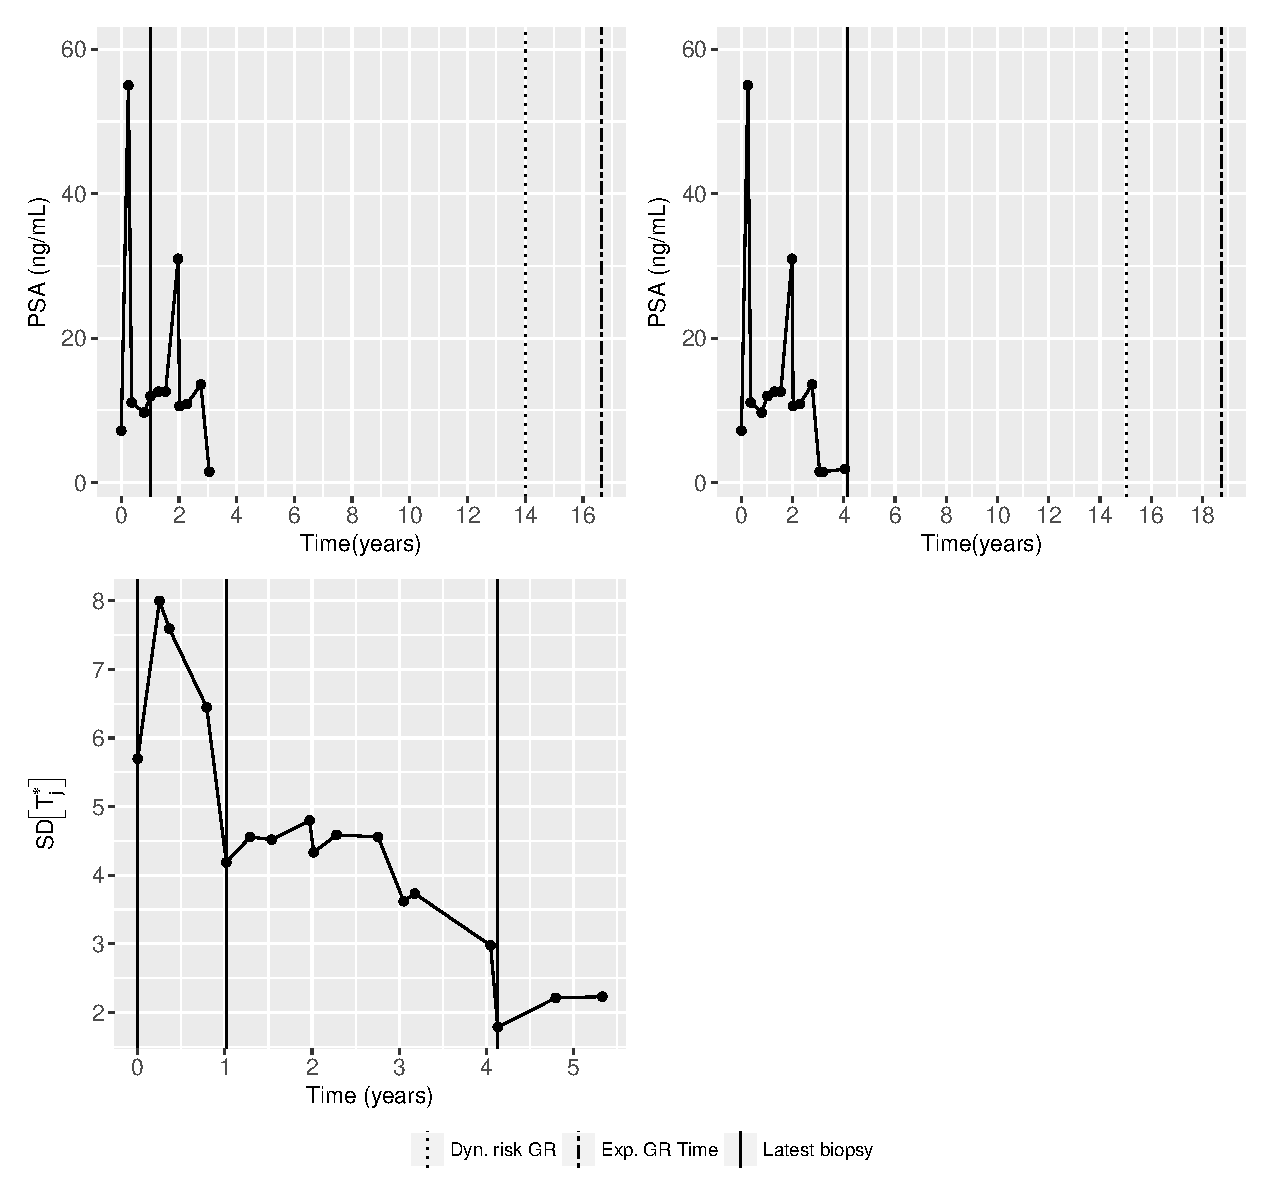
\includegraphics[width=\columnwidth]{images/prias_demo/case_911.eps}
}
\caption{Top panel: Evolution of PSA, history of repeat biopsies and corresponding personalized schedules for the first demonstration patient. Bottom Panel: History of repeat biopsies and $\mbox{SD}_g(T^*_j) = \sqrt{\mbox{var}_g(T^*_j)}$ over time for the first demonstration patient.}
\label{fig : prias_demo_pid_911}
\end{figure}

The demonstration of personalized schedules for the two other patients from the demonstration data set is presented in Web Appendix D of the supplementary material.